
\clearpage{}
\section{Projections}
\label{Inference:Projections}

This section gives the formal definition of type directed projections, which were introduced in \S\ref{System:Projections}. Syntactically, projections are a clean extension of the language described in \S\ref{Inference:Language}. Type inference for projections is a mostly-orthogonal extension to the system discussed thus far, though the handling of mutually recursive definitions requires careful ordering of the constraints considered by the inferencer. This section introduces type inference for projections, though we defer further discussion of mutual recursion and constraint ordering to \S\ref{inference:ordering}.

% -- Declarations
\subsubsection{Declarations}
\vspace{-1ex}
\begin{tabbing}
	MM	\= MM 	\= MM \= MMMMMMMMMMMMMMMMMMMM \= MMMMMMM \kill
		\> $\idecl$ \> $\to$ 	\> $\dots$ \\
		\>	\> \ $\mid$	\> $\kproject \ T \ \kwith \ \ov{l \sim x}$  	\> (projection declaration)
\end{tabbing}

% -- Terms
\vspace{-2em}
\subsubsection{Terms}
\vspace{-1ex}
\begin{tabbing}
	MM	\= MM 	\= MM \= MMMMMMMMMMMMMMMMMMMM \= MMMMMMM \kill
		\> $t$ 	\> $\to$ 	\> \ \dots \\
		\> 	\> \ $\mid$	\> \ $t_1 \odot l$	\> (projection) \\
		\> 	\> \ $\mid$	\> \ $t_1 \odot (l : c)$	\> (annotated projection)
\end{tabbing}

\subsubsection{Decl-Proj}

$$
\begin{aligned}
	\Gamma \judgea{decl} \kproject \ T \ \kwith \ \ov{l \ \sim x} \ :: \ \ov{l \sima{\:T} x}
\end{aligned}
$$

\vspace{-2em}
\subsubsection{Proj}

$$
\begin{aligned}
	\frac
	{ \Gamma \judge t :: T \ r \ \ov{\tau} \rhd \Omega \ ; \ e_2 \quad
	  \Gamma \judge x :: T \ r \ \ov{\tau} \lfuna{e_3 \ c_4} \tau' \rhd \Omega \ ; \ \bot \quad
	  l \sima{\:T} x \in \Gamma
	}
	{ \Gamma \judge t \odot l :: \tau' \rhd \Omega \ ; \ e_2 \lor e_3 }
\end{aligned}
$$

\begin{tabbing}
	MMMMMMMMMMMMMMMMMMMMM \= MMMMMMMMMMMMM \kill
	\hspace{12ex} 
	\includegraphics[scale=0.5]{3-Inference/fig/constraints/proj.eps} 
	\> 
	\begin{tabular}{lll}
		& $s_3$ 	& $= \rPROJ \ l \ s_2$ \\
		& $s_3$		& $= s_2 \lfuna{e_3 \ c_4} s_1$ \\
		& $e_1$		& $\tme e_2 \lor e_3$ \\
		\\ \\ \\ \\
	\end{tabular}
\end{tabbing}

\vspace{-4em}
\begin{tabbing}
MMMMMM \= MMMMMMM \= MMMMMMMMMM \= MMMMM \kill
	\> (projection)	 \> $\{ \ s_1 = \rPROJ \ l \ s_2,$ \> $s_2 = T \ \ov{s} \ \}$ \\
	\> \qq $\vvdash$ \> $\{ \ s_1 = \rINST \ s_v,$	  \> $s_2 = T \ \ov{s} \ \}$
	\\[1ex]
	\> \> \trm{where} \ \ $l \sima{T} v$
\end{tabbing}



A projection dictionary $\kproject \ T \ \kwith \ \ov{l \ \sim x}$ is associated with a particular type constructor $T$. The dictionary lists the names of the instance functions $\ov{x}$ that should be used to implement each of the projections labeled $\ov{l}$. Recall that the projection operator binds more tightly than function application, so $t_1 \ t_2 \ \odot \ \ifield$ should be read as $t_1 \ (t_2 \ \odot \ \ifield)$ The annotated projection $t_1 \odot (l : c)$ contains a closure variable $c$, and we will discuss how this is used in a moment.

The (Decl-Proj) rule introduces the bindings $\ov{l \sima{\:T} x}$ from the projection dictionary into the type environment.

The (Proj) rule says that to assign a type to the projection $t \ \odot \ l$, the expression $t$ must have a data type that includes an outer constructor $T$. There must be a binding $l \sima{T} x$ in the type environment showing which instance function $x$ to use to implement the projection. This instance function must take a value of the object type $T \ r \ \ov{\varphi}$ and return a value of the result type $\tau'$. We name the effect and closure of the instance function $e_3$ and $c_4$ respectively. Evaluation of the expression $t \ \odot \ l$ causes the instance function to be applied, so we have $e_3$ in the rule's conclusion.

In the list of constraints, $s_3 = \rPROJ \ l \ s_2$ says that we need to wait until the type of $s_2$ is known before we look up the instance function for $l$ from the corresponding projection dictionary. When this is done we can bind the type of the instance function to $s_3$. The constraint $s_3 = s_2 \lfuna{e_3 \ c_4} s_1$ requires the instance function to have an appropriate type. The last constraint gives the effect of the whole node.

We now discuss the meaning of the closure variable on an annotated projection. Firstly, recall that when we generate constraints for $\lambda$ abstractions, we need to know what free variables lie in their bodies. For example, if we have an annotated expression:

\qq\qq
\begin{tabular}{ll}
	& $\lambda (x : s_x). \ f \ x$	\\
\end{tabular}

With labeled syntax tree:

\begin{center}
\includegraphics[scale=0.5]{3-Inference/fig/projections/app-fx.eps}
\end{center}

This would lead to the following constraints:
\begin{tabbing}
MMMM 	\= MM \= MM \= MM \= MM \= MM \= MM \= MM \= MM \= MM \= MM \= MM \= MM \kill
	\> LAMBDA $\{ x \}$ \\
	\>	\> $s_0$ \> $= s_x \lfuna{e_1 \ c_0} s_1$ \\
	\>	\> $c_0$ \> $\tme f : s_f$ \\
	\>	\> $s_2$ \> $= s_f$ \\
	\>	\> $s_3$ \> $= s_x$
\end{tabbing}

The closure term $f : s_f$ is present because $f$ is free in the body of the abstraction. At runtime $f$ might be represented as a thunk which contains pointers to shared objects, and we use the closure term to account for this. 

Now, suppose that the body of the abstraction contained a projection instead:

\qq\qq
\begin{tabular}{ll}
	& $\lambda (x : s_x). \ x \ \odot \ l$ \\
\end{tabular}

\medskip
Until we have inferred the type of $x$ we won't know what instance function will be called, or what the closure of the body should be. If, during constraint reduction, we discover that the projection $x \ \odot \ l$ resolves to $g \ x$, then this tells us that it is $g$ that will be called at runtime. However, when generating constraints we can't use $c_0 \tme g : s_g$ as the closure constraint for the surrounding lambda abstraction, because we won't know about $g$ until the appropriate constraints are solved. Instead, we annotate the projection label with a fresh variable $c_1$, and use this as a place holder until the type of $x$ becomes known. Once the type of $x$ is known we can determine what instance function will be called, and then bind its closure to $c_1$.

\qq\qq
\begin{tabular}{ll}
	& $\lambda (x : s_x). \ x \ \odot \ (l : c_1)$ \\
\end{tabular}

The final task is to modify the constraint generation rules for lambda abstraction to take account of these new closure variables:

\subsubsection{Abs-Proj}
\begin{tabbing}
MMMMMMMMMMMMMMMMM \= MMMMMMMMMMMMM \kill
	\hspace{6em}\includegraphics[scale=0.5]{3-Inference/fig/constraints/lam}
	\> 
	\begin{tabular}{llll}
		\mc{4}{LAMBDA \ $\{ x \}$} \\
			& $s_1$ 	& $= s_x \lfuna{e_2 \ c_1} s_2$ \\
			& $c_1$		& $\tme \ y_0 : s_{y0} \ \lor \ y_1 : s_{y1} \ \lor \dots$ \\
			&		& $ \ \lor \ l_0 \ : c_0 \ \ \lor \ l_1 \ : c_1 \ \ \lor \dots$ \\
			&	& $\ \ \ \ \trm{where} \ y_n \hspace{5.4ex}\gets \ifv(t_2) \setminus x$ \\
			&	& $\ \ \ \ \hspace{2.6em} \ \ov{l_n : c_n} \ \ \gets \iclosAnnot(t_2)$ 
			\\[1ex]
			& \mc{2}{$\rbSLURP (t_2)$}
		\\ \\ \\ \\
	\end{tabular}
\end{tabbing}

\vspace{-4em}
The function $\iclosAnnot(t_2)$ simply collects the $(l:c)$ pairs from all expressions of the form $t \odot (l :c)$ present in term $t_2$. 

\subsection{Example: vectors}
\label{Inference:Projections:example}

The following program defines data types for vectors of two and three dimensions, along with projections that calculate their magnitudes. We have taken the liberty of using floating point numbers and infix operators without formally introducing them first, and have elided some insignificant details.

\begin{tabbing}
M 	\= MM \= MM \= MM \= MM \kill
	\> $\kdata \ \iVecTwo :: \% \to * \ \kwhere$ \\
	\> \> $\iMkVecTwo$ 	
		\> \> $:: \forall r_1 \ c_1
			. \iFloat \ r_1 \to \iFloat \ r_1 \lfuna{c_1} \iVecTwo \ r_1$ \\
	\> \>			\> \> $\rhd \ c_1 \tme x : r_1$ \
	\\[1ex]
	\> $\kdata \ \iVecThree :: \% \to * \ \kwhere$ \\
	\> \> $\iMkVecThree$	\> \> $:: \dots$
	\\[1ex]
	\> $\kproject \ \iVecTwo \ \kwith$ $\imagnitude \sim \ivecTwoMagnitude$ 
	\\[0.5ex]
	\> $\kproject \ \iVecThree \ \kwith$ $\imagnitude \sim \ivecThreeMagnitude$
	\\[1ex]
	\> $\klet$ 
		\> $\ivecTwoMagnitude$  $= \lambda v. \ \kcase \ v \ \kof$  $\iMkVecTwo \ x \ y \to \isqrt \ (x * x + y * y)$
	\\[0.5ex]
	\> 	\> $\ivecThreeMagnitude = \dots$ 
	\\[1ex]
	\>	\> $\ivec$ \> $= \ \iMkVecTwo \ 2.0 \ 3.0$ 
	\\[1ex]
	\> $\kin$ \ $\ivec \odot \imagnitude$
\end{tabbing}

Note that our full source language contains sugar that allows us to combine the projection dictionaries with the first two let-bindings. See \S\ref{System:Projections} for a description of this.

The point of this example is that the type inferencer will not be able to decide whether to use $\ivecTwoMagnitude$ or $\ivecThreeMagnitude$ to implement $\ivec \odot \imagnitude$ until it determines whether $\ivec$ is a $\iVecTwo$ or a $\iVecThree$. 

Here are the constraints for $\ivec \odot \imagnitude$, with $s_1$ being the type of the whole expression:
\begin{tabbing}
MMMM	\= MM \= MM \= MM \= MM \kill
	\> $s_3$ \> = PROJ \ $\imagnitude \ s_2$ \\
	\> $s_3$ \> $= s_2 \lfuna{e_{1a} \ c_{1a}} s_1$ \\
	\> $e_1$ \> $= e_2 \lor e_{1a}$ \\
	\> $s_2$ \> $= \rINST \ s_{\ivec}$
\end{tabbing}

Adding these to the type graph yields the following equivalence classes:
\begin{tabbing}
MMMM	\= MM 	\= MM 		\= MMMMMM 	\= MM \kill
	\> *1	\> $\sim$	\> $s_3$	\> $= \ \rPROJ \ \imagnitude \ s_2, 
							\quad s_2 \lfuna{e_{1a} \ c_{1a}} s_1$ \\
	\> *2	\> $\sim$	\> $s_2$	\> $= \ \rINST \ s_{\ivec}$ \\
	\> !1	\> $\sim$	\> $e_1$	\> $\tme \ e_2 \lor e_{1a}$
\end{tabbing}

Note the dependency between the constraint on $s_3$ and on $s_2$. Before we can crush $\rPROJ \ \imagnitude \ s_2$, we must wait until $s_2$ has been resolved to a concrete type. This requires that we first infer the type scheme for $\ivec$. Suppose this works out as:
\begin{tabbing}
MMMM	\= MM \= MM \kill
	\> $\ivec$ \> $:: \iVecTwo \ r_0$ 
\end{tabbing}
Instantiating this scheme (which is a no-op in this case) and adding it to the type graph gives:
\begin{tabbing}
MMMMM	\= MM 	\= MM 		\= MMMMMM 	\= MM \kill
	\> *1	\> $\sim$	\> $s_3$	\> $= \ \rPROJ \ \imagnitude \ s_2, 
							\quad s_2 \lfuna{e_{1a} \ c_{1a}} s_1$ \\
	\> *2	\> $\sim$	\> $s_2$	\> $= \ \iVecTwo \ r_0$ \\
	\> !1	\> $\sim$	\> $e_1$	\> $\tme \ e_2 \lor e_{1a}$
\end{tabbing}
Now that we have a constructor for $s_2$, we can lookup what projection instance function to use for $\imagnitude$ from the corresponding dictionary:
\begin{tabbing}
MMMM 	\= MM \= MM \= MM \= MM \kill
	\> $\kproject \ \iVecTwo \ \kwith$ $\imagnitude \sim \ivecTwoMagnitude$ 
\end{tabbing}
This tells us that $\imagnitude$ for $\iVecTwo$ types is implemented by $\ivecTwoMagnitude$, so we can crush the $\rPROJ$ constraint into an appropriate $\rINST$:
\begin{tabbing}
MMMMM	\= MM 	\= MM 		\= MMMMMM 	\= MM \kill
	\> *1	\> $\sim$	\> $s_3$	\> $= \ \rINST \ivecTwoMagnitude, 
							\quad s_2 \lfuna{e_{1a} \ c_{1a}} s_1$ \\
	\> *2	\> $\sim$	\> $s_2$	\> $= \ \iVecTwo \ r_0$ \\
	\> !1	\> $\sim$	\> $e_1$	\> $\tme \ e_2 \lor e_{1a}$
\end{tabbing}
Now we must wait until we have a type scheme for $\ivecTwoMagnitude$. Suppose this scheme works out to be:
\begin{tabbing}
MMMM	\= MM \= MM \kill
	\> $\ivecTwoMagnitude$ \\
	\> \> $:: \forall r_1 \ r_2 \ e_1. \ \iVecTwo \ r_1 \lfuna{e_1} \iFloat \ r_2$ \\
	\> \> $\rhd \ e_1 \tme \iRead \ r_1$ 
\end{tabbing}

\clearpage{}
Instantiating this scheme and adding it to the graph gives:
\begin{tabbing}
MMMMM	\= MM 	\= MM 		\= MMMMMM 	\= MM \kill
	\> *1	\> $\sim$	\> $s_3$	\> $= \ s_5 \lfuna{e_4} s_6, 
							\quad s_2 \lfuna{e_{1a} \ c_{1a}} s_1$ \\
	\> *2	\> $\sim$	\> $s_2$	\> $= \ \iVecTwo \ r_0$ \\
	\> *3	\> $\sim$	\> $s_5$	\> $= \ \iVecTwo \ r_4$ \\
	\> *4	\> $\sim$	\> $s_6$	\> $= \ \iFloat \ r_5$ \\
	\> !1	\> $\sim$	\> $e_1$	\> $\tme \ e_2 \lor e_{1a}$ \\
	\> !2	\> $\sim$	\> $e_4$	\> $\tme \ \iRead r_4$
\end{tabbing}
Performing the unification in *1 gives:
\begin{tabbing}
MMMMM	\= MM 	\= MM 		\= MMMMMM 		\= MM \kill
	\> *1	\> $\sim$	\> $s_3$		\> $= \ s_2 \lfuna{e_4 \ c_{1a}} s_1$ \\
	\> *2	\> $\sim$	\> $s_2, \ s_5$		\> $= \ \iVecTwo \ r_0$ \\
	\> *4	\> $\sim$	\> $s_1, \ s_6$		\> $= \ \iFloat \ r_5$ \\
	\> \%1	\> $\sim$	\> $r_0, \ r_4$	 \\	
	\> \ !1	\> $\sim$	\> $e_1$		\> $\tme \ e_2 \lor e_{1a}$ \\
	\> \ !2	\> $\sim$	\> $e_4, \ e_{1a}$	\> $\tme \ \iRead r_4$
\end{tabbing}

Inspecting the constraint on $s_1$ shows that the overall type of our program is $\iFloat \ r_5$. 

There are a few things we should note before moving on. Firstly, the type of a projection instance function is not required to be the same as another bound to the same label. For example, we could have defined $\ivecThreeMagnitude$ to return an $\iInt$ or a $\iList$, instead of a $\iFloat$ like with $\ivecTwoMagnitude$. Secondly, in general the inferencer must alternate between instantiating type schemes, performing unifications, and crushing projection constraints. Each $\rPROJ$ that is crushed results in an $\rINST$ constraint being added to the graph. This $\rINST$ constraint may need to be resolved, and some unifications performed, before we have the type that another $\rPROJ$ constraint is waiting for. This behaviour is common when the program includes chains of projections such as:

\qq\qq
\begin{tabular}{ll}
	$\iexp \odot \ifieldOne \odot \ifieldTwo \odot \ifieldThree$
\end{tabular}

The projections in this expression must be handled from left to right. We first determine the type of $\iexp$, use that to determine what instance function to use for $\ifieldOne$, add its type to the graph, and unify the resulting constraints. We can then use the solution to determine which instance function to use for $\ifieldTwo$, add its type to the graph, unify constraints, and so on.

In DDC we implement this behavior by maintaining several work sets of equivalence class identifiers. We have a set for classes that contain types needing to be unified; a set for projection constraints needing to be resolved, and a set for type class constraints needing to be crushed. The inferencer alternates between the various sets, working on one until nothing more can be done, then switching to another. If this process gets stuck, with one of the sets non-empty and no further progress possible, then this is a symptom of having an ambiguous projection constraint in the graph. 

\clearpage{}
\subsection{Ambiguous projections and type signatures}

Ambiguous projections are those that operate on values whose types are not constrained to include an outer constructor. For example, the projection in the following code is ambiguous:

\code{
	$\klet$ & $f = \lambda x. \ x \odot \imagnitude$ \\
	$\kin$ 	& \dots \\
}

The abstract syntax tree and constraints for the $f$ binding are:

\begin{tabbing}
MMMM \= MMMMMMMMMMMMMMM \= MMM \kill
	\>
	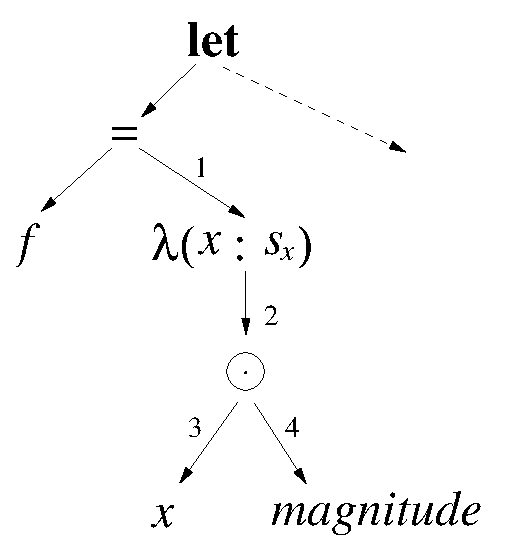
\includegraphics[scale=0.5]{3-Inference/fig/projections/ambiguous}
	\> 
	\begin{tabular}{lll}
		\mc{2}{LET $x$} \\
	 	\ \ \ \ \	
			& $s_f$ & $= s_1$ \\
		 	& $s_1$ & $= s_x \lfuna{e_2 \ c_1} s_2$ \\
	 		& $s_4$ & $= \rPROJ \ \imagnitude \ s_3$ \\
	 		& $s_4$ & $= s_3 \lfuna{e_4 \ c_5} s_2$ \\
			& $e_2$ & $\tme e_3 \lor e_4$ \\
	 		& $s_3$ & $= s_x$ \\
		\\ \\ \\ \\ \\ \\ \\ \\ \\
	\end{tabular}
\end{tabbing}

\vspace{-10em}

Adding these constraints to the type graph gives:
\begin{tabbing}
MMMMM	\= MM 	\= MM 		\= MMMMMM 		\= MM \kill
	\> *1	\> $\sim$	\> $s_f, \ s_1$		\> $= \ s_x \lfuna{e_2 \ c_{1}} s_2$ \\
	\> *2	\> $\sim$	\> $s_4$		\> $= \ \rPROJ \ \imagnitude \ s_x, \
								s_x \lfuna{e_4 \ c_5} s_2$ \\
	\> *3	\> $\sim$	\> $s_x, \ s_3$		\> $= \ \bot$ \\
	\> \ !1	\> $\sim$	\> $e_2$		\> $\tme e_3 \lor e_4$
\end{tabbing}

Note that *2 contains two separate type constraints, $\rPROJ \ \imagnitude \ s_x$ and $s_x \lfuna{e_5 \ c_5} s_2$. As we have no type constructor for $s_x$ we cannot crush the $\rPROJ$ constraint, and as we cannot represent both the $\rPROJ$ and function constraints as a normal form type we cannot make a type scheme for $f$. We can proceed no further, and in this situation our implementation reports an ambiguous projection error.

In future work we plan to investigate the possibility of assigning $f$ a type such as the following:

\code{
	$f$ 	& $:: \forall a \ b \ e_1 \ c_1. \ a \lfuna{e_1 \ c_1} b$ \\
		& $\rhd \ \iHasProj \ \imagnitude \ a \ (a \lfuna{e_1 \ c_1} b)$
}

In this type, the constraint $\iHasProj \ \imagnitude \ a \ (a \lfuna{e_1 \ c_1} b)$ says that $a$ can be any type that supports a projection $\imagnitude$ whose instance function has type $(a \lfuna{e_1 \ c_1} b)$. Such constraints are discussed in \cite{leigen:qualified-types-for-MLF}, and provide some aspects of a true record system \cite{remy:type-inference-for-records}.

For now, the programmer can fix ambiguous projections by supplying a type signature that constrains the type being projected. Importantly, they only need to supply enough information to allow the projection to be resolved. For example, the programmer could write:

\code{
	$\klet$ & $f :: \iVecTwo \to \iFloat$ \\
		& $f = \lambda x. \ x \odot \imagnitude$ \\
	$\kin$ 	& \dots \\
}

This signature does not contain quantifiers, region variables, or effect and closure information. The source desugarer uses the kinds of $\iVecTwo$, $\iFloat$, and the function constructor to determine that this information is missing. It then inserts fresh type variables in the appropriate positions:

\code{
	$f :: \iVecTwo \ r_6 \lfuna{e_7 \ c_8} \iFloat \ r_9$
}

This type is treated as a new constraint, and is added directly to the type graph:
\begin{tabbing}
MMMMM	\= MM 	\= MM 		\= MMMMMM 		\= MM \kill
	\> *1	\> $\sim$	\> $s_f, \ s_1$		\> $= \ s_x \lfuna{e_2 \ c_{1}} s_2, \
								s_5 \lfuna{e_7 \ c_8} s_6$\\
	\> *2	\> $\sim$	\> $s_4$		\> $= \ \rPROJ \ \imagnitude \ s_x, \
								s_x \lfuna{e_5 \ c_5} s_2$ \\
	\> *3	\> $\sim$	\> $s_x, \ s_3$		\> $= \ \bot$ \\
	\> *4	\> $\sim$	\> $s_5$		\> $= \ \iVecTwo \ r_6$ \\
	\> *5	\> $\sim$	\> $s_6$		\> $= \ \iFloat \ r_9$ \\
	\> \ !1	\> $\sim$	\> $e_1$		\> $\tme e_3 \lor e_4$
\end{tabbing}
The new constraint gives us enough information to resolve the projection in *2, though we need to perform the unification in *1 to expose it:
\begin{tabbing}
MMMMM	\= MM 	\= MM 		\= MMMMMM 		\= MM \kill
	\> *1	\> $\sim$	\> $s_f, \ s_1$		\> $= \ s_x \lfuna{e_2 \ c_{1}} s_2$ \\
	\> *2	\> $\sim$	\> $s_4$		\> $= \ \rPROJ \ \imagnitude \ s_x, \
								s_x \lfuna{e_5 \ c_5} s_2$ \\
	\> *3	\> $\sim$	\> $s_x, \ s_3, \ s_5$	\> $= \ \iVecTwo \ r_6$ \\
	\> *5	\> $\sim$	\> $s_2, \ s_6$		\> $= \ \iFloat \ r_9$ \\
	\> \ !1	\> $\sim$	\> $e_1$		\> $\tme \ e_3 \lor e_4$ \\
	\> \ !2 \> $\sim$	\> $e_2, \ e_7$		\> $\tme \ \bot$ \\
	\> \%1	\> $\sim$	\> $c_1, \ c_8$		\> $\tme \ \bot$ 
\end{tabbing}
Unifying the two function types in *1 has caused $s_x$ and $s_5$ to be identified. This in turn induces unification of classes *3 and *4. Class *3 now contains $\iVecTwo \ r_6$, which includes the constructor that the $\rPROJ$ constraint in *2 was waiting for. We can now lookup the type of the appropriate $\imagnitude$ instance function from the $\iVecTwo$ projection dictionary, crush the $\rPROJ$ constraint to an $\rINST$ of this type, and complete the inference process as per the example in \S\ref{Inference:Projections:example}



